

\section{MNIST 数据下载 }\label{mnist-ux6570ux636eux4e0bux8f7d}

源码:
\href{https://tensorflow.googlesource.com/tensorflow/+/master/tensorflow/g3doc/tutorials/mnist/}{tensorflow/g3doc/tutorials/mnist/}

本教程的目标是展示如何下载用于手写数字分类问题所要用到的(经典)MNIST数据集。

\subsection{教程 文件 }\label{ux6559ux7a0b-ux6587ux4ef6}

本教程需要使用以下文件:

\begin{longtable}[c]{@{}ll@{}}
\toprule
\begin{minipage}[b]{0.05\columnwidth}\raggedright\strut
文件
\strut\end{minipage} &
\begin{minipage}[b]{0.05\columnwidth}\raggedright\strut
目的
\strut\end{minipage}\tabularnewline
\midrule
\endhead
\begin{minipage}[t]{0.05\columnwidth}\raggedright\strut
\href{https://tensorflow.googlesource.com/tensorflow/+/master/tensorflow/g3doc/tutorials/mnist/input_data.py}{\texttt{input\_data.py}}
\strut\end{minipage} &
\begin{minipage}[t]{0.05\columnwidth}\raggedright\strut
下载用于训练和测试的MNIST数据集的源码
\strut\end{minipage}\tabularnewline
\bottomrule
\end{longtable}

\subsection{准备数据 }\label{ux51c6ux5907ux6570ux636e}

MNIST是在机器学习领域中的一个经典问题。该问题解决的是把28x28像素的灰度手写数字图片识别为相应的数字,其中数字的范围从0到9.

\begin{figure}[htbp]
\centering
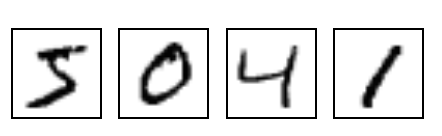
\includegraphics{../images/mnist_digits.png}
\caption{MNIST Digits}
\end{figure}

更多详情, 请参考 \href{http://yann.lecun.com/exdb/mnist/}{Yann LeCun's
MNIST page} 或
\href{http://colah.github.io/posts/2014-10-Visualizing-MNIST/}{Chris
Olah's visualizations of MNIST}.

\subsubsection{下载 }\label{ux4e0bux8f7d}

\href{http://yann.lecun.com/exdb/mnist/}{Yann LeCun's MNIST page}
也提供了训练集与测试集数据的下载。

\begin{longtable}[c]{@{}ll@{}}
\toprule
\begin{minipage}[b]{0.05\columnwidth}\raggedright\strut
文件
\strut\end{minipage} &
\begin{minipage}[b]{0.05\columnwidth}\raggedright\strut
内容
\strut\end{minipage}\tabularnewline
\midrule
\endhead
\begin{minipage}[t]{0.05\columnwidth}\raggedright\strut
\href{http://yann.lecun.com/exdb/mnist/train-images-idx3-ubyte.gz}{\texttt{train-images-idx3-ubyte.gz}}
\strut\end{minipage} &
\begin{minipage}[t]{0.05\columnwidth}\raggedright\strut
训练集图片 - 55000 张 训练图片, 5000 张 验证图片
\strut\end{minipage}\tabularnewline
\begin{minipage}[t]{0.05\columnwidth}\raggedright\strut
\href{http://yann.lecun.com/exdb/mnist/train-labels-idx1-ubyte.gz}{\texttt{train-labels-idx1-ubyte.gz}}
\strut\end{minipage} &
\begin{minipage}[t]{0.05\columnwidth}\raggedright\strut
训练集图片对应的数字标签
\strut\end{minipage}\tabularnewline
\begin{minipage}[t]{0.05\columnwidth}\raggedright\strut
\href{http://yann.lecun.com/exdb/mnist/t10k-images-idx3-ubyte.gz}{\texttt{t10k-images-idx3-ubyte.gz}}
\strut\end{minipage} &
\begin{minipage}[t]{0.05\columnwidth}\raggedright\strut
测试集图片 - 10000 张 图片
\strut\end{minipage}\tabularnewline
\begin{minipage}[t]{0.05\columnwidth}\raggedright\strut
\href{http://yann.lecun.com/exdb/mnist/t10k-labels-idx1-ubyte.gz}{\texttt{t10k-labels-idx1-ubyte.gz}}
\strut\end{minipage} &
\begin{minipage}[t]{0.05\columnwidth}\raggedright\strut
测试集图片对应的数字标签
\strut\end{minipage}\tabularnewline
\bottomrule
\end{longtable}

在 \texttt{input\_data.py} 文件中, \texttt{maybe\_download()}
函数可以确保这些训练数据下载到本地文件夹中。

文件夹的名字在 \texttt{fully\_connected\_feed.py}
文件的顶部由一个标记变量指定,你可以根据自己的需要进行修改。 \#\#\# 解压
与 重构

这些文件本身并没有使用标准的图片格式储存,并且需要使用\texttt{input\_data.py}文件中\texttt{extract\_images()}
和\texttt{extract\_labels()}函数来手动解压(页面中有相关说明)。

图片数据将被解压成2维的tensor:\texttt{{[}image\ index,\ pixel\ index{]}}
其中每一项表示某一图片中特定像素的强度值, 范围从 \texttt{{[}0,\ 255{]}}
到 \texttt{{[}-0.5,\ 0.5{]}}。 ``image index''代表数据集中图片的编号,
从0到数据集的上限值。``pixel index''代表该图片中像素点得个数,
从0到图片的像素上限值。

以\texttt{train-*}开头的文件中包括60000个样本,其中分割出55000个样本作为训练集,其余的5000个样本作为验证集。因为所有数据集中28x28像素的灰度图片的尺寸为784,所以训练集输出的tensor格式为\texttt{{[}55000,\ 784{]}}。

数字标签数据被解压称1维的tensor:
\texttt{{[}image\ index{]}},它定义了每个样本数值的类别分类。对于训练集的标签来说,这个数据规模就是:\texttt{{[}55000{]}}。

\subsubsection{数据集 对象 }\label{ux6570ux636eux96c6-ux5bf9ux8c61}

底层的源码将会执行下载、解压、重构图片和标签数据来组成以下的数据集对象:

\begin{longtable}[c]{@{}ll@{}}
\toprule
数据集 & 目的\tabularnewline
\midrule
\endhead
\texttt{data\_sets.train} & 55000 组 图片和标签,
用于训练。\tabularnewline
\texttt{data\_sets.validation} & 5000 组 图片和标签,
用于迭代验证训练的准确性。\tabularnewline
\texttt{data\_sets.test} & 10000 组 图片和标签,
用于最终测试训练的准确性。\tabularnewline
\bottomrule
\end{longtable}

执行\texttt{read\_data\_sets()}函数将会返回一个\texttt{DataSet}实例,其中包含了以上三个数据集。函数\texttt{DataSet.next\_batch()}是用于获取以\texttt{batch\_size}为大小的一个元组,其中包含了一组图片和标签,该元组会被用于当前的TensorFlow运算会话中。

\begin{Shaded}
\begin{Highlighting}[]
\NormalTok{images_feed, labels_feed }\OperatorTok{=} \NormalTok{data_set.next_batch(FLAGS.batch_size)}
\end{Highlighting}
\end{Shaded}

原文地址:\href{https://github.com/tensorflow/tensorflow/blob/master/tensorflow/g3doc/tutorials/mnist/download/index.md}{MNIST
Data Download} 翻译:\href{https://github.com/btpeter}{btpeter}
校对:waiwaizheng